\PassOptionsToPackage{unicode=true}{hyperref} % options for packages loaded elsewhere
\PassOptionsToPackage{hyphens}{url}
%
\documentclass[12pt,ignorenonframetext,aspectratio=169]{beamer}
\usepackage{pgfpages}
\setbeamertemplate{caption}[numbered]
\setbeamertemplate{caption label separator}{: }
\setbeamercolor{caption name}{fg=normal text.fg}
\beamertemplatenavigationsymbolsempty
% Prevent slide breaks in the middle of a paragraph:
\widowpenalties 1 10000
\raggedbottom
\setbeamertemplate{part page}{
\centering
\begin{beamercolorbox}[sep=16pt,center]{part title}
  \usebeamerfont{part title}\insertpart\par
\end{beamercolorbox}
}
\setbeamertemplate{section page}{
\centering
\begin{beamercolorbox}[sep=12pt,center]{part title}
  \usebeamerfont{section title}\insertsection\par
\end{beamercolorbox}
}
\setbeamertemplate{subsection page}{
\centering
\begin{beamercolorbox}[sep=8pt,center]{part title}
  \usebeamerfont{subsection title}\insertsubsection\par
\end{beamercolorbox}
}
\AtBeginPart{
  \frame{\partpage}
}
\AtBeginSection{
  \ifbibliography
  \else
    \frame{\sectionpage}
  \fi
}
\AtBeginSubsection{
  \frame{\subsectionpage}
}
\usepackage{lmodern}
\usepackage{amssymb,amsmath}
\usepackage{ifxetex,ifluatex}
\usepackage{fixltx2e} % provides \textsubscript
\ifnum 0\ifxetex 1\fi\ifluatex 1\fi=0 % if pdftex
  \usepackage[T1]{fontenc}
  \usepackage[utf8]{inputenc}
  \usepackage{textcomp} % provides euro and other symbols
\else % if luatex or xelatex
  \usepackage{unicode-math}
  \defaultfontfeatures{Ligatures=TeX,Scale=MatchLowercase}
\fi
\usetheme[]{metropolis}
% use upquote if available, for straight quotes in verbatim environments
\IfFileExists{upquote.sty}{\usepackage{upquote}}{}
% use microtype if available
\IfFileExists{microtype.sty}{%
\usepackage[]{microtype}
\UseMicrotypeSet[protrusion]{basicmath} % disable protrusion for tt fonts
}{}
\IfFileExists{parskip.sty}{%
\usepackage{parskip}
}{% else
\setlength{\parindent}{0pt}
\setlength{\parskip}{6pt plus 2pt minus 1pt}
}
\usepackage{hyperref}
\hypersetup{
            pdftitle={Bayesian hierarchical models},
            pdfauthor={Bruno Nicenboim / Shravan Vasishth},
            pdfborder={0 0 0},
            breaklinks=true}
\urlstyle{same}  % don't use monospace font for urls
\newif\ifbibliography
\usepackage{color}
\usepackage{fancyvrb}
\newcommand{\VerbBar}{|}
\newcommand{\VERB}{\Verb[commandchars=\\\{\}]}
\DefineVerbatimEnvironment{Highlighting}{Verbatim}{commandchars=\\\{\}}
% Add ',fontsize=\small' for more characters per line
\usepackage{framed}
\definecolor{shadecolor}{RGB}{248,248,248}
\newenvironment{Shaded}{\begin{snugshade}}{\end{snugshade}}
\newcommand{\AlertTok}[1]{\textcolor[rgb]{0.94,0.16,0.16}{#1}}
\newcommand{\AnnotationTok}[1]{\textcolor[rgb]{0.56,0.35,0.01}{\textbf{\textit{#1}}}}
\newcommand{\AttributeTok}[1]{\textcolor[rgb]{0.77,0.63,0.00}{#1}}
\newcommand{\BaseNTok}[1]{\textcolor[rgb]{0.00,0.00,0.81}{#1}}
\newcommand{\BuiltInTok}[1]{#1}
\newcommand{\CharTok}[1]{\textcolor[rgb]{0.31,0.60,0.02}{#1}}
\newcommand{\CommentTok}[1]{\textcolor[rgb]{0.56,0.35,0.01}{\textit{#1}}}
\newcommand{\CommentVarTok}[1]{\textcolor[rgb]{0.56,0.35,0.01}{\textbf{\textit{#1}}}}
\newcommand{\ConstantTok}[1]{\textcolor[rgb]{0.00,0.00,0.00}{#1}}
\newcommand{\ControlFlowTok}[1]{\textcolor[rgb]{0.13,0.29,0.53}{\textbf{#1}}}
\newcommand{\DataTypeTok}[1]{\textcolor[rgb]{0.13,0.29,0.53}{#1}}
\newcommand{\DecValTok}[1]{\textcolor[rgb]{0.00,0.00,0.81}{#1}}
\newcommand{\DocumentationTok}[1]{\textcolor[rgb]{0.56,0.35,0.01}{\textbf{\textit{#1}}}}
\newcommand{\ErrorTok}[1]{\textcolor[rgb]{0.64,0.00,0.00}{\textbf{#1}}}
\newcommand{\ExtensionTok}[1]{#1}
\newcommand{\FloatTok}[1]{\textcolor[rgb]{0.00,0.00,0.81}{#1}}
\newcommand{\FunctionTok}[1]{\textcolor[rgb]{0.00,0.00,0.00}{#1}}
\newcommand{\ImportTok}[1]{#1}
\newcommand{\InformationTok}[1]{\textcolor[rgb]{0.56,0.35,0.01}{\textbf{\textit{#1}}}}
\newcommand{\KeywordTok}[1]{\textcolor[rgb]{0.13,0.29,0.53}{\textbf{#1}}}
\newcommand{\NormalTok}[1]{#1}
\newcommand{\OperatorTok}[1]{\textcolor[rgb]{0.81,0.36,0.00}{\textbf{#1}}}
\newcommand{\OtherTok}[1]{\textcolor[rgb]{0.56,0.35,0.01}{#1}}
\newcommand{\PreprocessorTok}[1]{\textcolor[rgb]{0.56,0.35,0.01}{\textit{#1}}}
\newcommand{\RegionMarkerTok}[1]{#1}
\newcommand{\SpecialCharTok}[1]{\textcolor[rgb]{0.00,0.00,0.00}{#1}}
\newcommand{\SpecialStringTok}[1]{\textcolor[rgb]{0.31,0.60,0.02}{#1}}
\newcommand{\StringTok}[1]{\textcolor[rgb]{0.31,0.60,0.02}{#1}}
\newcommand{\VariableTok}[1]{\textcolor[rgb]{0.00,0.00,0.00}{#1}}
\newcommand{\VerbatimStringTok}[1]{\textcolor[rgb]{0.31,0.60,0.02}{#1}}
\newcommand{\WarningTok}[1]{\textcolor[rgb]{0.56,0.35,0.01}{\textbf{\textit{#1}}}}
\usepackage{longtable,booktabs}
\usepackage{caption}
% These lines are needed to make table captions work with longtable:
\makeatletter
\def\fnum@table{\tablename~\thetable}
\makeatother
\usepackage{graphicx,grffile}
\makeatletter
\def\maxwidth{\ifdim\Gin@nat@width>\linewidth\linewidth\else\Gin@nat@width\fi}
\def\maxheight{\ifdim\Gin@nat@height>\textheight\textheight\else\Gin@nat@height\fi}
\makeatother
% Scale images if necessary, so that they will not overflow the page
% margins by default, and it is still possible to overwrite the defaults
% using explicit options in \includegraphics[width, height, ...]{}
\setkeys{Gin}{width=\maxwidth,height=\maxheight,keepaspectratio}
\setlength{\emergencystretch}{3em}  % prevent overfull lines
\providecommand{\tightlist}{%
  \setlength{\itemsep}{0pt}\setlength{\parskip}{0pt}}
\setcounter{secnumdepth}{5}

% set default figure placement to htbp
\makeatletter
\def\fps@figure{htbp}
\makeatother

  \setbeamercolor{frametitle}{bg=gray}
  \hypersetup{colorlinks,citecolor=orange,filecolor=red,linkcolor=brown,urlcolor=blue}
% \setsansfont[BoldFont={FiraSans-Bold.ttf}]{FiraSans-Light.ttf}
% \setmonofont{FiraMono-Regular.ttf}
\usepackage[sfdefault]{FiraSans}
\newcommand{\hideFromPandoc}[1]{#1}
         \hideFromPandoc{
             \let\Begin\begin
             \let\End\end
         }

\setbeamerfont{caption}{size=\scriptsize}

\title{Bayesian hierarchical models}
\author{Bruno Nicenboim / Shravan Vasishth}
\date{2020-03-14}

\begin{document}
\frame{\titlepage}

\begin{frame}
\tableofcontents[hideallsubsections]
\end{frame}
\hypertarget{bayesian-hierarchical-models-also-known-as-multilevel-or-mixed-effects-models}{%
\section{Bayesian hierarchical models (also known as multilevel or mixed-effects models)}\label{bayesian-hierarchical-models-also-known-as-multilevel-or-mixed-effects-models}}

\small

\normalsize

\begin{frame}{The N400 effect (hierarchical normal likelihood)}
\protect\hypertarget{the-n400-effect-hierarchical-normal-likelihood}{}

In the EEG literature, it has been shown that words with low-predictability are accompanied by an \emph{N400 effect} in comparison with high-predictable words, this is a relative negativity that peaks around 300-500 after word onset over central parietal scalp sites (first noticed in Kutas and Hillyard 1980, for semantic anomalies and in 1984 for low predictable word; for a review: Kutas and Federmeier 2011).

\begin{enumerate}
\tightlist
\item
  Example from DeLong, Urbach, and Kutas (2005)

  \begin{enumerate}
  [a.]
  \tightlist
  \item
    The day was breezy so the boy went outside to fly a kite.\\
  \item
    The day was breezy so the boy went outside to fly an airplane.
  \end{enumerate}
\end{enumerate}

\end{frame}

\begin{frame}

\small

\begin{figure}

{\centering 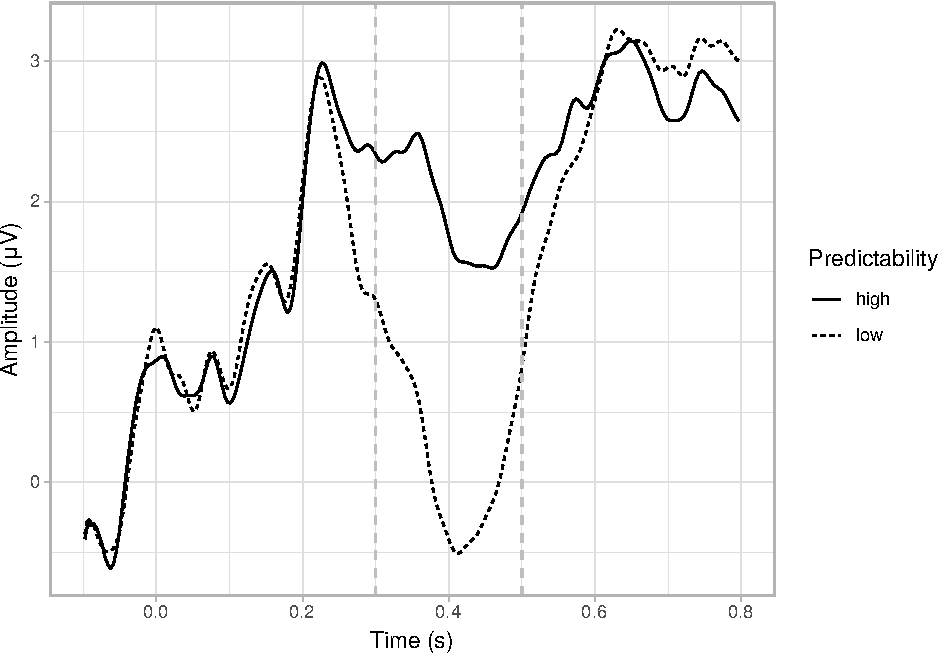
\includegraphics[width=0.8\linewidth]{cc_figure/N400noun-1} 

}

\caption{(ref:mot)}\label{fig:mot}
\end{figure}

\normalsize

\end{frame}

\begin{frame}

\begin{itemize}
\tightlist
\item
  We simplify the high-dimensional EEG data by focusing on the average amplitude of the EEG signal at the typical spatio-temporal window of the N400.
\item
  We focus on the N400 effect for nouns from a subset of the data from Nieuwland et al. (2018). (To speed-up computation, we'll restrict the dataset to the participants from the Edinburgh lab)
\end{itemize}

\end{frame}

\begin{frame}[fragile]

\scriptsize

\begin{Shaded}
\begin{Highlighting}[]
\NormalTok{df_eeg_data <-}\StringTok{ }\KeywordTok{read_tsv}\NormalTok{(}\StringTok{"data/public_noun_data.txt"}\NormalTok{) }\OperatorTok
\StringTok{  }\KeywordTok{filter}\NormalTok{(lab }\OperatorTok{==}\StringTok{ "edin"}\NormalTok{) }\OperatorTok
\StringTok{  }\KeywordTok{mutate}\NormalTok{(}\DataTypeTok{c_cloze =}\NormalTok{ cloze }\OperatorTok{/}\StringTok{ }\DecValTok{100} \OperatorTok{-}\StringTok{ }\KeywordTok{mean}\NormalTok{(cloze }\OperatorTok{/}\StringTok{ }\DecValTok{100}\NormalTok{))}
\NormalTok{df_eeg_data}\OperatorTok{$}\NormalTok{c_cloze }\OperatorTok\StringTok{ }\KeywordTok{summary}\NormalTok{()}
\end{Highlighting}
\end{Shaded}

\begin{verbatim}
##    Min. 1st Qu.  Median    Mean 3rd Qu.    Max. 
##   -0.47   -0.44    0.03    0.00    0.43    0.53
\end{verbatim}

\normalsize

\end{frame}

\begin{frame}

One nice aspect of this dataset is that the dependent variable is roughly normally distributed:

\small

\begin{figure}
\centering
\includegraphics{05-hierarchical-slides_files/figure-beamer/unnamed-chunk-2-1.pdf}
\caption{\label{fig:unnamed-chunk-2}Histogram of the N400 averages for every trial in gray; density plot of a normal distribution in red.}
\end{figure}

\normalsize

\end{frame}

\begin{frame}{A complete pooling model}
\protect\hypertarget{a-complete-pooling-model}{}

We'll start from the simplest model which is basically a linear regression. \textbf{Note that this model is incorrect for these data due to point 2 below.}

\begin{itemize}
\tightlist
\item
  Model \(M_{cp}\) assumptions:
\end{itemize}

\begin{enumerate}
\tightlist
\item
  EEG averages for the N400 spatiotemporal window are normally distributed.
\item
  Observations are \emph{independent}.
\item
  There is a linear relationship between cloze and the EEG average for the trial.
\end{enumerate}

\end{frame}

\begin{frame}

\begin{itemize}
\tightlist
\item
  Likelihood:
\end{itemize}

\begin{equation}
   signal_n \sim Normal(\alpha + c\_cloze_n \cdot \beta,\sigma)
   \end{equation}

\begin{itemize}
\tightlist
\item
  Priors:
\end{itemize}

\begin{equation}
 \begin{aligned}
 \alpha &\sim Normal(0,10)\\
 \beta  &\sim Normal(0,10)\\
 \sigma  &\sim Normal_{+}(0,50)
 \end{aligned}
 \end{equation}

\end{frame}

\begin{frame}[fragile]{Fitting the model}
\protect\hypertarget{fitting-the-model}{}

\small

\begin{Shaded}
\begin{Highlighting}[]
\NormalTok{fit_N400_cp <-}\StringTok{ }\KeywordTok{brm}\NormalTok{(n400 }\OperatorTok{~}\StringTok{ }\NormalTok{c_cloze,}
  \DataTypeTok{prior =}
    \KeywordTok{c}\NormalTok{(}\KeywordTok{prior}\NormalTok{(}\KeywordTok{normal}\NormalTok{(}\DecValTok{0}\NormalTok{, }\DecValTok{10}\NormalTok{), }\DataTypeTok{class =}\NormalTok{ Intercept),}
      \KeywordTok{prior}\NormalTok{(}\KeywordTok{normal}\NormalTok{(}\DecValTok{0}\NormalTok{, }\DecValTok{10}\NormalTok{), }\DataTypeTok{class =}\NormalTok{ b),}
      \KeywordTok{prior}\NormalTok{(}\KeywordTok{normal}\NormalTok{(}\DecValTok{0}\NormalTok{, }\DecValTok{50}\NormalTok{), }\DataTypeTok{class =}\NormalTok{ sigma)),}
  \DataTypeTok{data =}\NormalTok{ df_eeg_data}
\NormalTok{)}
\end{Highlighting}
\end{Shaded}

\normalsize

\end{frame}

\begin{frame}[fragile]

\scriptsize

\begin{Shaded}
\begin{Highlighting}[]
\NormalTok{fit_N400_cp}
\end{Highlighting}
\end{Shaded}

\begin{verbatim}
##  Family: gaussian 
##   Links: mu = identity; sigma = identity 
## Formula: n400 ~ c_cloze 
##    Data: df_eeg_data (Number of observations: 2827) 
## Samples: 4 chains, each with iter = 2000; warmup = 1000; thin = 1;
##          total post-warmup samples = 4000
## 
## Population-Level Effects: 
##           Estimate Est.Error l-95% CI u-95% CI Rhat
## Intercept     3.66      0.23     3.22     4.10 1.00
## c_cloze       2.26      0.55     1.19     3.33 1.00
##           Bulk_ESS Tail_ESS
## Intercept     4301     3214
## c_cloze       4038     3036
## 
## Family Specific Parameters: 
##       Estimate Est.Error l-95% CI u-95% CI Rhat
## sigma    11.84      0.16    11.54    12.15 1.00
##       Bulk_ESS Tail_ESS
## sigma     4865     3060
## 
## Samples were drawn using sampling(NUTS). For each parameter, Bulk_ESS
## and Tail_ESS are effective sample size measures, and Rhat is the potential
## scale reduction factor on split chains (at convergence, Rhat = 1).
\end{verbatim}

\normalsize

\end{frame}

\begin{frame}[fragile]

\small

\begin{Shaded}
\begin{Highlighting}[]
\KeywordTok{plot}\NormalTok{(fit_N400_cp)}
\end{Highlighting}
\end{Shaded}

\includegraphics{05-hierarchical-slides_files/figure-beamer/unnamed-chunk-5-1.pdf}

\normalsize

\end{frame}

\begin{frame}{No pooling model}
\protect\hypertarget{no-pooling-model}{}

\begin{itemize}
\tightlist
\item
  Model \(M_{np}\) assumptions:
\end{itemize}

\begin{enumerate}
\tightlist
\item
  EEG averages for the N400 spatio-temporal window are normally distributed.
\item
  Observations depend \emph{completely} on the participant. (Participants have nothing in common.)
\item
  There is a linear relationship between cloze and the EEG average for the trial.
\end{enumerate}

\end{frame}

\begin{frame}

\begin{itemize}
\tightlist
\item
  Likelihood:
\end{itemize}

\begin{equation}
 signal_n \sim Normal( \alpha_{i[n]} + c\_cloze_n \cdot \beta_{i[n]},\sigma)
 \end{equation}

\begin{itemize}
\tightlist
\item
  Priors:
\end{itemize}

\begin{equation}
 \begin{aligned}
 \alpha_i &\sim Normal(0,10)\\
 \beta_i  &\sim Normal(0,10)\\
 \sigma  &\sim Normal_+(0,50)
 \end{aligned}
 \end{equation}

\end{frame}

\begin{frame}[fragile]

We fit it in brms by removing the common intercept with \texttt{0\ +} and thus having an intercept and effect for each level of \texttt{subject}:

\scriptsize

\begin{Shaded}
\begin{Highlighting}[]
\NormalTok{fit_N400_np <-}\StringTok{ }\KeywordTok{brm}\NormalTok{(n400 }\OperatorTok{~}\StringTok{ }\DecValTok{0} \OperatorTok{+}
\StringTok{                     }\KeywordTok{factor}\NormalTok{(subject) }\OperatorTok{+}\StringTok{ }\NormalTok{c_cloze}\OperatorTok{:}\KeywordTok{factor}\NormalTok{(subject),}
                 \DataTypeTok{prior =}
                     \KeywordTok{c}\NormalTok{(}\KeywordTok{prior}\NormalTok{(}\KeywordTok{normal}\NormalTok{(}\DecValTok{0}\NormalTok{, }\DecValTok{10}\NormalTok{), }\DataTypeTok{class =}\NormalTok{ b),}
                       \KeywordTok{prior}\NormalTok{(}\KeywordTok{normal}\NormalTok{(}\DecValTok{0}\NormalTok{, }\DecValTok{50}\NormalTok{), }\DataTypeTok{class =}\NormalTok{ sigma)),}
                 \DataTypeTok{data =}\NormalTok{ df_eeg_data)}
\end{Highlighting}
\end{Shaded}

\normalsize

\end{frame}

\begin{frame}[fragile]

\vspace{.1in}

\tiny

\begin{Shaded}
\begin{Highlighting}[]
\NormalTok{fit_N400_np}
\end{Highlighting}
\end{Shaded}

\begin{verbatim}
##  Family: gaussian 
##   Links: mu = identity; sigma = identity 
## Formula: n400 ~ 0 + factor(subject) + c_cloze:factor(subject) 
##    Data: df_eeg_data (Number of observations: 2827) 
## Samples: 4 chains, each with iter = 2000; warmup = 1000; thin = 1;
##          total post-warmup samples = 4000
## 
## Population-Level Effects: 
##                             Estimate Est.Error
## factorsubjectedin1              5.35      1.35
## factorsubjectedin10             2.72      1.43
## factorsubjectedin11             2.71      1.33
## factorsubjectedin12             7.61      1.30
## factorsubjectedin13             1.30      1.31
## factorsubjectedin14            -0.07      1.35
## factorsubjectedin15             1.20      1.31
## factorsubjectedin16             5.59      1.33
## factorsubjectedin17             2.54      1.28
## factorsubjectedin18             2.52      1.31
## factorsubjectedin19             5.52      1.36
## factorsubjectedin2              3.38      1.36
## factorsubjectedin20             2.61      1.26
## factorsubjectedin21            -0.53      1.34
## factorsubjectedin23             2.84      1.32
## factorsubjectedin24            -0.13      1.38
## factorsubjectedin25             6.29      1.42
## factorsubjectedin26             1.34      1.39
## factorsubjectedin27             7.65      1.30
## factorsubjectedin28             6.27      1.30
## factorsubjectedin3              1.85      1.35
## factorsubjectedin30             1.66      1.29
## factorsubjectedin31             5.61      1.26
## factorsubjectedin32             4.18      1.31
## factorsubjectedin33             2.55      1.36
## factorsubjectedin34             0.78      1.37
## factorsubjectedin36             0.38      1.32
## factorsubjectedin37             0.99      1.32
## factorsubjectedin38             3.48      1.29
## factorsubjectedin39             6.10      1.35
## factorsubjectedin4              7.64      1.30
## factorsubjectedin40             4.03      1.32
## factorsubjectedin5              8.12      1.30
## factorsubjectedin6              6.34      1.28
## factorsubjectedin7              5.29      1.26
## factorsubjectedin8              2.23      1.36
## factorsubjectedin9              4.97      1.38
## factorsubjectedin1:c_cloze     -1.63      2.93
## factorsubjectedin10:c_cloze    -2.23      3.39
## factorsubjectedin11:c_cloze    -0.39      3.36
## factorsubjectedin12:c_cloze     2.86      3.12
## factorsubjectedin13:c_cloze    -1.10      2.91
## factorsubjectedin14:c_cloze     7.73      3.03
## factorsubjectedin15:c_cloze    -1.47      3.17
## factorsubjectedin16:c_cloze     7.50      3.35
## factorsubjectedin17:c_cloze    -0.86      2.93
## factorsubjectedin18:c_cloze     4.88      3.02
## factorsubjectedin19:c_cloze     2.96      3.08
## factorsubjectedin2:c_cloze      1.14      3.02
## factorsubjectedin20:c_cloze     3.65      3.19
## factorsubjectedin21:c_cloze    -2.08      3.02
## factorsubjectedin23:c_cloze     4.41      3.22
## factorsubjectedin24:c_cloze    -1.60      3.23
## factorsubjectedin25:c_cloze     2.28      3.21
## factorsubjectedin26:c_cloze     2.91      3.18
## factorsubjectedin27:c_cloze     2.63      3.02
## factorsubjectedin28:c_cloze    -1.58      3.20
## factorsubjectedin3:c_cloze      6.53      3.26
## factorsubjectedin30:c_cloze    -0.87      3.02
## factorsubjectedin31:c_cloze     2.63      3.18
## factorsubjectedin32:c_cloze     5.00      3.18
## factorsubjectedin33:c_cloze    -3.32      3.01
## factorsubjectedin34:c_cloze     0.37      3.16
## factorsubjectedin36:c_cloze     0.13      3.20
## factorsubjectedin37:c_cloze     6.61      3.05
## factorsubjectedin38:c_cloze     2.07      2.94
## factorsubjectedin39:c_cloze     5.75      3.26
## factorsubjectedin4:c_cloze      2.72      3.22
## factorsubjectedin40:c_cloze     1.53      3.15
## factorsubjectedin5:c_cloze      0.08      2.91
## factorsubjectedin6:c_cloze     -0.14      2.97
## factorsubjectedin7:c_cloze      9.04      3.25
## factorsubjectedin8:c_cloze      7.27      3.29
## factorsubjectedin9:c_cloze      5.33      3.03
##                             l-95% CI u-95% CI Rhat
## factorsubjectedin1              2.76     8.07 1.00
## factorsubjectedin10            -0.08     5.61 1.00
## factorsubjectedin11             0.06     5.28 1.00
## factorsubjectedin12             5.06    10.09 1.00
## factorsubjectedin13            -1.32     3.86 1.00
## factorsubjectedin14            -2.69     2.60 1.00
## factorsubjectedin15            -1.37     3.80 1.00
## factorsubjectedin16             3.03     8.20 1.00
## factorsubjectedin17             0.06     4.99 1.00
## factorsubjectedin18            -0.09     5.06 1.00
## factorsubjectedin19             2.83     8.12 1.00
## factorsubjectedin2              0.65     6.06 1.00
## factorsubjectedin20             0.16     5.15 1.00
## factorsubjectedin21            -3.16     2.10 1.00
## factorsubjectedin23             0.27     5.36 1.00
## factorsubjectedin24            -2.84     2.57 1.00
## factorsubjectedin25             3.49     9.03 1.00
## factorsubjectedin26            -1.40     4.07 1.00
## factorsubjectedin27             5.18    10.21 1.00
## factorsubjectedin28             3.74     8.85 1.00
## factorsubjectedin3             -0.82     4.39 1.00
## factorsubjectedin30            -0.83     4.21 1.00
## factorsubjectedin31             3.18     8.07 1.00
## factorsubjectedin32             1.63     6.74 1.00
## factorsubjectedin33            -0.11     5.27 1.00
## factorsubjectedin34            -1.90     3.41 1.00
## factorsubjectedin36            -2.15     2.98 1.00
## factorsubjectedin37            -1.58     3.52 1.00
## factorsubjectedin38             0.87     6.01 1.00
## factorsubjectedin39             3.42     8.74 1.00
## factorsubjectedin4              5.13    10.21 1.00
## factorsubjectedin40             1.44     6.62 1.00
## factorsubjectedin5              5.62    10.69 1.00
## factorsubjectedin6              3.82     8.82 1.00
## factorsubjectedin7              2.77     7.77 1.00
## factorsubjectedin8             -0.47     4.88 1.00
## factorsubjectedin9              2.31     7.69 1.00
## factorsubjectedin1:c_cloze     -7.62     4.08 1.00
## factorsubjectedin10:c_cloze    -8.75     4.51 1.00
## factorsubjectedin11:c_cloze    -6.86     6.17 1.00
## factorsubjectedin12:c_cloze    -3.36     8.89 1.00
## factorsubjectedin13:c_cloze    -6.75     4.70 1.00
## factorsubjectedin14:c_cloze     1.71    13.27 1.00
## factorsubjectedin15:c_cloze    -7.71     4.90 1.00
## factorsubjectedin16:c_cloze     0.92    14.19 1.00
## factorsubjectedin17:c_cloze    -6.65     4.87 1.00
## factorsubjectedin18:c_cloze    -0.99    10.74 1.00
## factorsubjectedin19:c_cloze    -3.18     9.05 1.00
## factorsubjectedin2:c_cloze     -4.72     7.04 1.00
## factorsubjectedin20:c_cloze    -2.65     9.93 1.00
## factorsubjectedin21:c_cloze    -8.09     3.85 1.00
## factorsubjectedin23:c_cloze    -2.01    10.75 1.00
## factorsubjectedin24:c_cloze    -7.97     4.74 1.00
## factorsubjectedin25:c_cloze    -4.03     8.48 1.00
## factorsubjectedin26:c_cloze    -3.16     9.20 1.00
## factorsubjectedin27:c_cloze    -3.35     8.52 1.00
## factorsubjectedin28:c_cloze    -7.98     4.51 1.00
## factorsubjectedin3:c_cloze      0.14    12.96 1.00
## factorsubjectedin30:c_cloze    -6.74     5.16 1.00
## factorsubjectedin31:c_cloze    -3.70     8.83 1.00
## factorsubjectedin32:c_cloze    -1.31    11.00 1.00
## factorsubjectedin33:c_cloze    -9.35     2.53 1.00
## factorsubjectedin34:c_cloze    -5.68     6.63 1.00
## factorsubjectedin36:c_cloze    -6.11     6.27 1.00
## factorsubjectedin37:c_cloze     0.72    12.75 1.00
## factorsubjectedin38:c_cloze    -3.69     7.90 1.00
## factorsubjectedin39:c_cloze    -0.69    12.12 1.00
## factorsubjectedin4:c_cloze     -3.76     9.07 1.00
## factorsubjectedin40:c_cloze    -4.58     7.70 1.00
## factorsubjectedin5:c_cloze     -5.47     5.72 1.00
## factorsubjectedin6:c_cloze     -6.01     5.70 1.00
## factorsubjectedin7:c_cloze      2.82    15.34 1.00
## factorsubjectedin8:c_cloze      1.01    13.68 1.00
## factorsubjectedin9:c_cloze     -0.76    11.33 1.00
##                             Bulk_ESS Tail_ESS
## factorsubjectedin1              5970     2900
## factorsubjectedin10             5934     2583
## factorsubjectedin11             6624     2612
## factorsubjectedin12             4962     2774
## factorsubjectedin13             6384     3034
## factorsubjectedin14             6755     2603
## factorsubjectedin15             5564     2780
## factorsubjectedin16             6426     2992
## factorsubjectedin17             5556     3159
## factorsubjectedin18             6865     2945
## factorsubjectedin19             5495     3062
## factorsubjectedin2              7682     2866
## factorsubjectedin20             5966     2827
## factorsubjectedin21             7364     2833
## factorsubjectedin23             6510     2910
## factorsubjectedin24             6134     2521
## factorsubjectedin25             6139     3005
## factorsubjectedin26             5887     2809
## factorsubjectedin27             6173     3057
## factorsubjectedin28             6351     2772
## factorsubjectedin3              6060     2819
## factorsubjectedin30             6568     3158
## factorsubjectedin31             5738     2905
## factorsubjectedin32             5711     3018
## factorsubjectedin33             5888     2835
## factorsubjectedin34             6101     3083
## factorsubjectedin36             6109     2952
## factorsubjectedin37             5831     3003
## factorsubjectedin38             6133     2958
## factorsubjectedin39             6169     3080
## factorsubjectedin4              5341     2708
## factorsubjectedin40             5094     2885
## factorsubjectedin5              5261     2682
## factorsubjectedin6              6131     2554
## factorsubjectedin7              4806     3085
## factorsubjectedin8              6102     2784
## factorsubjectedin9              5893     3001
## factorsubjectedin1:c_cloze      5715     2456
## factorsubjectedin10:c_cloze     5902     3155
## factorsubjectedin11:c_cloze     5492     2860
## factorsubjectedin12:c_cloze     6251     2941
## factorsubjectedin13:c_cloze     5923     3116
## factorsubjectedin14:c_cloze     5236     2910
## factorsubjectedin15:c_cloze     5006     2957
## factorsubjectedin16:c_cloze     5380     2677
## factorsubjectedin17:c_cloze     6266     2861
## factorsubjectedin18:c_cloze     5844     2872
## factorsubjectedin19:c_cloze     5005     3322
## factorsubjectedin2:c_cloze      5796     2903
## factorsubjectedin20:c_cloze     5542     2639
## factorsubjectedin21:c_cloze     5719     2966
## factorsubjectedin23:c_cloze     5704     2908
## factorsubjectedin24:c_cloze     5652     3144
## factorsubjectedin25:c_cloze     5181     2928
## factorsubjectedin26:c_cloze     5431     2844
## factorsubjectedin27:c_cloze     5314     2867
## factorsubjectedin28:c_cloze     6456     2653
## factorsubjectedin3:c_cloze      5626     2687
## factorsubjectedin30:c_cloze     6810     2960
## factorsubjectedin31:c_cloze     6804     2975
## factorsubjectedin32:c_cloze     4971     2652
## factorsubjectedin33:c_cloze     5542     2990
## factorsubjectedin34:c_cloze     6160     2922
## factorsubjectedin36:c_cloze     5919     2791
## factorsubjectedin37:c_cloze     6684     2913
## factorsubjectedin38:c_cloze     5409     3266
## factorsubjectedin39:c_cloze     5782     3047
## factorsubjectedin4:c_cloze      6225     2810
## factorsubjectedin40:c_cloze     5618     2651
## factorsubjectedin5:c_cloze      5987     3145
## factorsubjectedin6:c_cloze      6113     3152
## factorsubjectedin7:c_cloze      5740     3130
## factorsubjectedin8:c_cloze      6492     3189
## factorsubjectedin9:c_cloze      5548     3145
## 
## Family Specific Parameters: 
##       Estimate Est.Error l-95% CI u-95% CI Rhat
## sigma    11.63      0.15    11.33    11.93 1.00
##       Bulk_ESS Tail_ESS
## sigma     6026     3173
## 
## Samples were drawn using sampling(NUTS). For each parameter, Bulk_ESS
## and Tail_ESS are effective sample size measures, and Rhat is the potential
## scale reduction factor on split chains (at convergence, Rhat = 1).
\end{verbatim}

\normalsize

\end{frame}

\begin{frame}[fragile]

We plot the estimates using \texttt{bayesplot}.

\bigskip

\scriptsize

\begin{Shaded}
\begin{Highlighting}[]
\CommentTok{# I first peek at the internal names of the parameters.}
\CommentTok{# parnames(fit_N400_np)}
\NormalTok{ind_effects_np <-}\StringTok{ }\KeywordTok{paste0}\NormalTok{(}
  \StringTok{"b_factorsubject"}\NormalTok{,}
  \KeywordTok{unique}\NormalTok{(df_eeg_data}\OperatorTok{$}\NormalTok{subject), }\StringTok{":c_cloze"}
\NormalTok{)}
\KeywordTok{mcmc_intervals}\NormalTok{(fit_N400_np,}
  \DataTypeTok{pars =}\NormalTok{ ind_effects_np,}
  \DataTypeTok{prob =} \FloatTok{0.8}\NormalTok{,}
  \DataTypeTok{prob_outer =} \FloatTok{0.95}\NormalTok{,}
  \DataTypeTok{point_est =} \StringTok{"mean"}
\NormalTok{)}
\end{Highlighting}
\end{Shaded}

\normalsize

\end{frame}

\begin{frame}

\small

\includegraphics{05-hierarchical-slides_files/figure-beamer/unnamed-chunk-9-1.pdf}

\normalsize

\end{frame}

\begin{frame}[fragile]

We can then calculate the average of the \(\beta\)'s, even though the model doesn't assume that there's one common \(\beta\):

\footnotesize

\begin{Shaded}
\begin{Highlighting}[]
\NormalTok{average_beta_across_subj <-}
\StringTok{    }\KeywordTok{posterior_samples}\NormalTok{(fit_N400_np,}
                      \DataTypeTok{pars =}\NormalTok{ ind_effects_np) }\OperatorTok
\StringTok{    }\KeywordTok{rowMeans}\NormalTok{()}
\KeywordTok{c}\NormalTok{(}\DataTypeTok{mean=}\KeywordTok{mean}\NormalTok{(average_beta_across_subj),}
  \KeywordTok{quantile}\NormalTok{(average_beta_across_subj,}
           \KeywordTok{c}\NormalTok{(.}\DecValTok{025}\NormalTok{,.}\DecValTok{975}\NormalTok{)))}
\end{Highlighting}
\end{Shaded}

\begin{verbatim}
## mean 2.5%  98% 
##  2.2  1.2  3.2
\end{verbatim}

\normalsize

\end{frame}

\begin{frame}{Varying intercept and varying slopes model (\(M_{v}\))}
\protect\hypertarget{varying-intercept-and-varying-slopes-model-m_v}{}

\begin{itemize}
\tightlist
\item
  Model \(M_{v}\) assumptions:
\end{itemize}

\begin{enumerate}
\tightlist
\item
  EEG averages for the N400 spatio-temporal window are normally distributed.
\item
  Each subject deviates to some extent (this is made precise below) from the grand mean and from the mean effect of predictability.
\item
  There is a linear relationship between cloze and the EEG average for the trial.
\end{enumerate}

\end{frame}

\begin{frame}

\begin{itemize}
\tightlist
\item
  Likelihood:
\end{itemize}

\begin{equation}
 signal_n \sim Normal(\alpha + u_{0,i[n]} + c\_cloze_n \cdot (\beta+ u_{1,i[n]}),\sigma)
 \end{equation}

\begin{itemize}
\tightlist
\item
  Prior:
\end{itemize}

\begin{equation}
 \begin{aligned}
 \alpha &\sim Normal(0,10)\\
 \beta  &\sim Normal(0,10)\\
 u_0 &\sim Normal(0,\tau_{u_0})\\
 u_1 &\sim Normal(0,\tau_{u_1})\\
 \tau_{u_0} &\sim Normal_+(0,20) \\
 \tau_{u_1} &\sim Normal_+(0,20) \\
 \sigma  &\sim Normal_+(0,50)
 \end{aligned}
 \end{equation}

\end{frame}

\begin{frame}

Some important (and sometimes confusing) points:

\begin{itemize}
\tightlist
\item
  Why does \(u\) have a mean of 0?
\end{itemize}

Because we want \(u\) to capture only differences between subjects, we could achieve the same by assuming that

\begin{equation}
\begin{aligned}
\mu_n &= \alpha_{i[n]} + \beta_{i[n]} \cdot c\_cloze_n \text{and} \\
\alpha_i &\sim Normal(\alpha,\tau_{u_0})\\
\alpha &\sim Normal(0,10)\\
\beta_i &\sim Normal(\beta,\tau_{u_1})\\
\beta &\sim Normal(0,10)
\end{aligned}
\end{equation}

And in fact, that's another common way to write the model.

\end{frame}

\begin{frame}

\begin{itemize}
\tightlist
\item
  Why do the adjustments \(u\) have a normal distribution?
\end{itemize}

Mostly because of ``convention'', that's the way it's implemented in most frequentist mixed models.

But also because if we don't know anything about the distribution besides its mean and variance, the normal distribution is the most conservative assumption (see also chapter 9 of McElreath 2015).

\end{frame}

\begin{frame}[fragile]

Let's see how we need to set up the priors:

\scriptsize

\begin{Shaded}
\begin{Highlighting}[]
\KeywordTok{get_prior}\NormalTok{(n400 }\OperatorTok{~}\StringTok{ }\NormalTok{c_cloze }\OperatorTok{+}\StringTok{ }\NormalTok{(c_cloze }\OperatorTok{||}\StringTok{ }\NormalTok{subject), }\DataTypeTok{data =}\NormalTok{ df_eeg_data)}
\end{Highlighting}
\end{Shaded}

\begin{verbatim}
##                 prior     class      coef   group resp
## 1                             b                       
## 2                             b   c_cloze             
## 3 student_t(3, 4, 11) Intercept                       
## 4 student_t(3, 0, 11)        sd                       
## 5                            sd           subject     
## 6                            sd   c_cloze subject     
## 7                            sd Intercept subject     
## 8 student_t(3, 0, 11)     sigma                       
##   dpar nlpar bound
## 1                 
## 2                 
## 3                 
## 4                 
## 5                 
## 6                 
## 7                 
## 8
\end{verbatim}

\normalsize

\end{frame}

\begin{frame}[fragile]

\scriptsize

\begin{Shaded}
\begin{Highlighting}[]
\NormalTok{fit_N400_v <-}\StringTok{ }\KeywordTok{brm}\NormalTok{(n400 }\OperatorTok{~}\StringTok{ }\NormalTok{c_cloze }\OperatorTok{+}\StringTok{ }\NormalTok{(c_cloze }\OperatorTok{||}\StringTok{ }\NormalTok{subject),}
               \DataTypeTok{prior =}
                 \KeywordTok{c}\NormalTok{(}\KeywordTok{prior}\NormalTok{(}\KeywordTok{normal}\NormalTok{(}\DecValTok{0}\NormalTok{, }\DecValTok{10}\NormalTok{), }\DataTypeTok{class =}\NormalTok{ Intercept),}
                   \KeywordTok{prior}\NormalTok{(}\KeywordTok{normal}\NormalTok{(}\DecValTok{0}\NormalTok{, }\DecValTok{10}\NormalTok{), }\DataTypeTok{class =}\NormalTok{ b, }\DataTypeTok{coef =}\NormalTok{ c_cloze),}
                   \KeywordTok{prior}\NormalTok{(}\KeywordTok{normal}\NormalTok{(}\DecValTok{0}\NormalTok{, }\DecValTok{50}\NormalTok{), }\DataTypeTok{class =}\NormalTok{ sigma),}
                   \KeywordTok{prior}\NormalTok{(}\KeywordTok{normal}\NormalTok{(}\DecValTok{0}\NormalTok{, }\DecValTok{20}\NormalTok{), }\DataTypeTok{class =}\NormalTok{ sd, }\DataTypeTok{coef =}\NormalTok{ Intercept,}
                         \DataTypeTok{group =}\NormalTok{ subject),}
                   \KeywordTok{prior}\NormalTok{(}\KeywordTok{normal}\NormalTok{(}\DecValTok{0}\NormalTok{, }\DecValTok{20}\NormalTok{), }\DataTypeTok{class =}\NormalTok{ sd, }\DataTypeTok{coef =}\NormalTok{ c_cloze,}
                         \DataTypeTok{group =}\NormalTok{ subject)}
\NormalTok{                   ),}
               \DataTypeTok{data =}\NormalTok{ df_eeg_data)}
\end{Highlighting}
\end{Shaded}

\normalsize

\end{frame}

\begin{frame}[fragile]

\vspace{.1in}

\scriptsize

\begin{Shaded}
\begin{Highlighting}[]
\NormalTok{fit_N400_v}
\end{Highlighting}
\end{Shaded}

\begin{verbatim}
##  Family: gaussian 
##   Links: mu = identity; sigma = identity 
## Formula: n400 ~ c_cloze + (c_cloze || subject) 
##    Data: df_eeg_data (Number of observations: 2827) 
## Samples: 4 chains, each with iter = 2000; warmup = 1000; thin = 1;
##          total post-warmup samples = 4000
## 
## Group-Level Effects: 
## ~subject (Number of levels: 37) 
##               Estimate Est.Error l-95% CI u-95% CI
## sd(Intercept)     2.20      0.37     1.56     3.01
## sd(c_cloze)       1.56      0.90     0.08     3.42
##               Rhat Bulk_ESS Tail_ESS
## sd(Intercept) 1.00     1392     1893
## sd(c_cloze)   1.00     1130     1437
## 
## Population-Level Effects: 
##           Estimate Est.Error l-95% CI u-95% CI Rhat
## Intercept     3.65      0.42     2.80     4.48 1.00
## c_cloze       2.32      0.62     1.07     3.58 1.00
##           Bulk_ESS Tail_ESS
## Intercept     1298     1755
## c_cloze       3809     2735
## 
## Family Specific Parameters: 
##       Estimate Est.Error l-95% CI u-95% CI Rhat
## sigma    11.64      0.16    11.33    11.96 1.00
##       Bulk_ESS Tail_ESS
## sigma     5129     2816
## 
## Samples were drawn using sampling(NUTS). For each parameter, Bulk_ESS
## and Tail_ESS are effective sample size measures, and Rhat is the potential
## scale reduction factor on split chains (at convergence, Rhat = 1).
\end{verbatim}

\normalsize

\end{frame}

\begin{frame}[fragile]

\small

\begin{Shaded}
\begin{Highlighting}[]
\KeywordTok{plot}\NormalTok{(fit_N400_v, }\DataTypeTok{N =} \DecValTok{6}\NormalTok{)}
\end{Highlighting}
\end{Shaded}

\includegraphics{05-hierarchical-slides_files/figure-beamer/unnamed-chunk-14-1.pdf}

\normalsize

\end{frame}

\begin{frame}[fragile]{Individual effects}
\protect\hypertarget{individual-effects}{}

\scriptsize

\begin{Shaded}
\begin{Highlighting}[]
\CommentTok{# parnames(m_N400_v)}
\NormalTok{ind_effects_v <-}\StringTok{ }\KeywordTok{paste0}\NormalTok{(}\StringTok{"r_subject["}\NormalTok{, }\KeywordTok{unique}\NormalTok{(eeg_data}\OperatorTok{$}\NormalTok{subject), }\StringTok{",ccloze]"}\NormalTok{)}
\KeywordTok{mcmc_intervals}\NormalTok{(fit_N400_v,}
  \DataTypeTok{pars =}\NormalTok{ ind_effects_v,}
  \DataTypeTok{prob =} \FloatTok{0.8}\NormalTok{,}
  \DataTypeTok{prob_outer =} \FloatTok{0.95}\NormalTok{,}
  \DataTypeTok{point_est =} \StringTok{"mean"}
\NormalTok{)}
\end{Highlighting}
\end{Shaded}

\normalsize

\end{frame}

\begin{frame}

\vspace{.1in}

\small

\includegraphics{05-hierarchical-slides_files/figure-beamer/unnamed-chunk-16-1.pdf}

\normalsize

\end{frame}

\begin{frame}{Shrinkage}
\protect\hypertarget{shrinkage}{}

\small

\includegraphics[width=2\linewidth]{05-hierarchical-slides_files/figure-beamer/comparison-1}

\normalsize

\end{frame}

\begin{frame}{Correlated varying intercept varying slopes model (\(M_{h}\))}
\protect\hypertarget{sec:mcvivs}{}

\begin{itemize}
\tightlist
\item
  In \(M_h\), we model the EEG data with the following assumptions:
\end{itemize}

\begin{enumerate}
\tightlist
\item
  EEG averages for the N400 spatio-temporal window are normally distributed.
\item
  Some aspects of the signal voltage and the effect of predictability on the signal depend on the participant, and these two might be correlated, i.e., we assume random intercept, slope and correlation by-subject.
\item
  There is a linear relationship between cloze and the EEG average for the trial.
\end{enumerate}

\end{frame}

\begin{frame}

\begin{itemize}
\tightlist
\item
  Likelihood:
\end{itemize}

\begin{equation}
  signal_n \sim Normal(\alpha + u_{i[n],0} + c\_cloze_n \cdot  (\beta + u_{i[n],1}),\sigma)
  \end{equation}

We need to have priors on the adjustments for intercept and slopes, \(u_{,0-1}\).

\begin{itemize}
\tightlist
\item
  Priors:
  \begin{equation}
   \begin{aligned}
   \alpha & \sim Normal(0,10) \\
   \beta  & \sim Normal(0,10) \\
    \sigma  &\sim Normal_+(0,50)\\
    {\begin{pmatrix}
    u_{i,0} \\
    u_{i,1}
    \end{pmatrix}}
   &\sim {\mathcal {N}}
    \left(
   {\begin{pmatrix} 
    0\\
    0
   \end{pmatrix}}
   ,\boldsymbol{\Sigma_u} \right)
   \end{aligned}
   \end{equation}
\end{itemize}

\end{frame}

\begin{frame}

\begin{equation}
\boldsymbol{\Sigma_u} = 
{\begin{pmatrix} 
\tau_{u_0}^2 & \rho_u \tau_{u_0} \tau_{u_1} \\ 
\rho_u \tau_{u_0} \tau_{u_1} & \tau_{u_1}^2
\end{pmatrix}}
\end{equation}

\end{frame}

\begin{frame}

And now we need priors for the \(\tau_u\)s and for \(\rho_u\):

\begin{equation}
\begin{aligned}
\tau_{u_0} &\sim Normal_+(0,20)\\
\tau_{u_1} &\sim Normal_+(0,20)\\
\rho_u &\sim LKJcorr(2) 
\end{aligned}
\end{equation}

\end{frame}

\begin{frame}

\vspace{.1in}



\small

\begin{figure}
\includegraphics[width=.48\linewidth]{05-hierarchical-slides_files/figure-beamer/lkjviz-1} \includegraphics[width=.48\linewidth]{05-hierarchical-slides_files/figure-beamer/lkjviz-2} \includegraphics[width=.48\linewidth]{05-hierarchical-slides_files/figure-beamer/lkjviz-3} \includegraphics[width=.48\linewidth]{05-hierarchical-slides_files/figure-beamer/lkjviz-4} \caption{Visualization of the LKJ prior with four different values of the \(\eta\) parameter.}\label{fig:lkjviz}
\end{figure}

\normalsize

\end{frame}

\begin{frame}[fragile]

Let's see how we need to set up the priors:

\scriptsize

\begin{Shaded}
\begin{Highlighting}[]
\KeywordTok{get_prior}\NormalTok{(n400 }\OperatorTok{~}\StringTok{ }\NormalTok{c_cloze }\OperatorTok{+}\StringTok{ }\NormalTok{(c_cloze }\OperatorTok{|}\StringTok{ }\NormalTok{subject), }\DataTypeTok{data =}\NormalTok{ df_eeg_data)}
\end{Highlighting}
\end{Shaded}

\begin{verbatim}
##                  prior     class      coef   group
## 1                              b                  
## 2                              b   c_cloze        
## 3               lkj(1)       cor                  
## 4                            cor           subject
## 5  student_t(3, 4, 11) Intercept                  
## 6  student_t(3, 0, 11)        sd                  
## 7                             sd           subject
## 8                             sd   c_cloze subject
## 9                             sd Intercept subject
## 10 student_t(3, 0, 11)     sigma                  
##    resp dpar nlpar bound
## 1                       
## 2                       
## 3                       
## 4                       
## 5                       
## 6                       
## 7                       
## 8                       
## 9                       
## 10
\end{verbatim}

\normalsize

\end{frame}

\begin{frame}[fragile]{Fitting the model}
\protect\hypertarget{fitting-the-model-1}{}

\scriptsize

\begin{Shaded}
\begin{Highlighting}[]
\NormalTok{fit_N400_h <-}\StringTok{ }\KeywordTok{brm}\NormalTok{(n400 }\OperatorTok{~}\StringTok{ }\NormalTok{c_cloze }\OperatorTok{+}\StringTok{ }\NormalTok{(c_cloze }\OperatorTok{|}\StringTok{ }\NormalTok{subject),}
                  \DataTypeTok{prior =}
                      \KeywordTok{c}\NormalTok{(}\KeywordTok{prior}\NormalTok{(}\KeywordTok{normal}\NormalTok{(}\DecValTok{0}\NormalTok{, }\DecValTok{10}\NormalTok{), }\DataTypeTok{class =}\NormalTok{ Intercept),}
                        \KeywordTok{prior}\NormalTok{(}\KeywordTok{normal}\NormalTok{(}\DecValTok{0}\NormalTok{, }\DecValTok{10}\NormalTok{), }\DataTypeTok{class =}\NormalTok{ b, }\DataTypeTok{coef =}\NormalTok{ c_cloze),}
                        \KeywordTok{prior}\NormalTok{(}\KeywordTok{normal}\NormalTok{(}\DecValTok{0}\NormalTok{, }\DecValTok{50}\NormalTok{), }\DataTypeTok{class =}\NormalTok{ sigma),}
                        \KeywordTok{prior}\NormalTok{(}\KeywordTok{normal}\NormalTok{(}\DecValTok{0}\NormalTok{, }\DecValTok{20}\NormalTok{), }\DataTypeTok{class =}\NormalTok{ sd, }\DataTypeTok{coef =}\NormalTok{ Intercept,}
                              \DataTypeTok{group =}\NormalTok{ subject),}
                        \KeywordTok{prior}\NormalTok{(}\KeywordTok{normal}\NormalTok{(}\DecValTok{0}\NormalTok{, }\DecValTok{20}\NormalTok{), }\DataTypeTok{class =}\NormalTok{ sd, }\DataTypeTok{coef =}\NormalTok{ c_cloze,}
                              \DataTypeTok{group =}\NormalTok{ subject),}
                        \KeywordTok{prior}\NormalTok{(}\KeywordTok{lkj}\NormalTok{(}\DecValTok{2}\NormalTok{), }\DataTypeTok{class =}\NormalTok{ cor,}
                              \DataTypeTok{group=}\NormalTok{ subject)),}
              \DataTypeTok{data =}\NormalTok{ df_eeg_data)}
\end{Highlighting}
\end{Shaded}

\normalsize

\end{frame}

\begin{frame}[fragile]

\scriptsize

\begin{Shaded}
\begin{Highlighting}[]
\NormalTok{fit_N400_h}
\end{Highlighting}
\end{Shaded}

\begin{verbatim}
##  Family: gaussian 
##   Links: mu = identity; sigma = identity 
## Formula: n400 ~ c_cloze + (c_cloze | subject) 
##    Data: df_eeg_data (Number of observations: 2827) 
## Samples: 4 chains, each with iter = 2000; warmup = 1000; thin = 1;
##          total post-warmup samples = 4000
## 
## Group-Level Effects: 
## ~subject (Number of levels: 37) 
##                        Estimate Est.Error l-95% CI
## sd(Intercept)              2.22      0.36     1.57
## sd(c_cloze)                1.46      0.90     0.08
## cor(Intercept,c_cloze)     0.17      0.36    -0.60
##                        u-95% CI Rhat Bulk_ESS Tail_ESS
## sd(Intercept)              2.97 1.00     1418     2688
## sd(c_cloze)                3.36 1.00     1128     1724
## cor(Intercept,c_cloze)     0.79 1.00     3602     2786
## 
## Population-Level Effects: 
##           Estimate Est.Error l-95% CI u-95% CI Rhat
## Intercept     3.62      0.44     2.77     4.47 1.00
## c_cloze       2.34      0.60     1.17     3.53 1.00
##           Bulk_ESS Tail_ESS
## Intercept     1724     2353
## c_cloze       3725     2671
## 
## Family Specific Parameters: 
##       Estimate Est.Error l-95% CI u-95% CI Rhat
## sigma    11.64      0.15    11.34    11.94 1.00
##       Bulk_ESS Tail_ESS
## sigma     6972     3334
## 
## Samples were drawn using sampling(NUTS). For each parameter, Bulk_ESS
## and Tail_ESS are effective sample size measures, and Rhat is the potential
## scale reduction factor on split chains (at convergence, Rhat = 1).
\end{verbatim}

\normalsize

\end{frame}

\begin{frame}[fragile]

\small

\begin{Shaded}
\begin{Highlighting}[]
\KeywordTok{plot}\NormalTok{(fit_N400_h, }\DataTypeTok{N =} \DecValTok{6}\NormalTok{)}
\end{Highlighting}
\end{Shaded}

\includegraphics{05-hierarchical-slides_files/figure-beamer/unnamed-chunk-20-1.pdf}

\normalsize

\end{frame}

\begin{frame}{Why should we take the trouble of fitting a Bayesian hierarchical model?}
\protect\hypertarget{why-should-we-take-the-trouble-of-fitting-a-bayesian-hierarchical-model}{}

\begin{itemize}
\tightlist
\item
  We can better characterize the generative process by adding the relevant clusters in our data (participants, items, maybe labs, etc)
\item
  The same approach we used here can be used to extend any parameter of any model:

  \begin{itemize}
  \tightlist
  \item
    (generalized) linear models
  \item
    non-linear/cognitive models
  \end{itemize}
\end{itemize}

\end{frame}

\begin{frame}{How much structure should we add to our statistical models?}
\protect\hypertarget{how-much-structure-should-we-add-to-our-statistical-models}{}

\begin{block}{The level of complexity depends on}

\begin{enumerate}
\tightlist
\item
  the answers we are looking for
\item
  the size of the data at hand\\
\item
  our computing power
\item
  our domain and experimental knowledge.
\end{enumerate}

\vspace{.3in}

\begin{quote}
``Simplification is essential, but it comes at a cost, and real understanding depends in part on understanding the effects of the simplification'' McClelland (2009)
\end{quote}

\end{block}

\end{frame}

\begin{frame}{References}
\protect\hypertarget{references}{}

\hypertarget{refs}{}
\leavevmode\hypertarget{ref-delongProbabilisticWordPreactivation2005}{}%
DeLong, Katherine A, Thomas P Urbach, and Marta Kutas. 2005. ``Probabilistic Word Pre-Activation During Language Comprehension Inferred from Electrical Brain Activity.'' \emph{Nature Neuroscience} 8 (8): 1117--21. \url{https://doi.org/10.1038/nn1504}.

\leavevmode\hypertarget{ref-kutasThirtyYearsCounting2011}{}%
Kutas, Marta, and Kara D. Federmeier. 2011. ``Thirty Years and Counting: Finding Meaning in the N400 Componentof the Event-Related Brain Potential (ERP).'' \emph{Annual Review of Psychology} 62 (1): 621--47. \url{https://doi.org/10.1146/annurev.psych.093008.131123}.

\leavevmode\hypertarget{ref-kutasReadingSenselessSentences1980}{}%
Kutas, Marta, and Steven A Hillyard. 1980. ``Reading Senseless Sentences: Brain Potentials Reflect Semantic Incongruity.'' \emph{Science} 207 (4427): 203--5. \url{https://doi.org/10.1126/science.7350657}.

\leavevmode\hypertarget{ref-kutasBrainPotentialsReading1984}{}%
---------. 1984. ``Brain Potentials During Reading Reflect Word Expectancy and Semantic Association.'' \emph{Nature} 307 (5947): 161--63. \url{https://doi.org/10.1038/307161a0}.

\leavevmode\hypertarget{ref-mcclellandPlaceModelingCognitive2009}{}%
McClelland, James L. 2009. ``The Place of Modeling in Cognitive Science.'' \emph{Topics in Cognitive Science} 1 (1): 11--38. \url{https://doi.org/10.1111/j.1756-8765.2008.01003.x}.

\leavevmode\hypertarget{ref-mcelreath2015statistical}{}%
McElreath, Richard. 2015. \emph{Statistical Rethinking: A Bayesian Course with R Examples}. Chapman; Hall/CRC.

\leavevmode\hypertarget{ref-nieuwlandLargescaleReplicationStudy2018}{}%
Nieuwland, Mante S, Stephen Politzer-Ahles, Evelien Heyselaar, Katrien Segaert, Emily Darley, Nina Kazanina, Sarah Von Grebmer Zu Wolfsthurn, et al. 2018. ``Large-Scale Replication Study Reveals a Limit on Probabilistic Prediction in Language Comprehension.'' \emph{eLife} 7. \url{https://doi.org/10.7554/eLife.33468}.

\end{frame}

\end{document}
